% Semantic Afterlife manuscript (Stage 7), Russian translation of paper/main.tex.
% English source is canonical. Numbers, run_id comments, and citations match.
% Every quantitative claim carries a same-line LaTeX comment: artifact path + run_id.
% Cite only VERIFIED entries in docs/literature/related-work.md (see paper/refs.bib).
\documentclass[11pt,a4paper]{article}

\usepackage[T1,T2A]{fontenc}
\usepackage[utf8]{inputenc}
\usepackage[english,russian]{babel}
\usepackage[margin=1in]{geometry}
\usepackage{graphicx}
\usepackage{booktabs}
\usepackage{amsmath}
\usepackage{amssymb}
\usepackage{natbib}
\usepackage[unicode,hidelinks]{hyperref}
\usepackage{setspace}
\usepackage{microtype}

\graphicspath{{../artifacts/}}
\setstretch{1.08}

\title{Семантическая загробная жизнь:\\
occupancy lock'а после ухода промпта из окна}
\author{Adam Cage}
\date{}

\begin{document}
\maketitle

\begin{abstract}
Языковая модель, чей вход усечён до последних $W$ сгенерированных токенов,
продолжает работу после того, как исходный промпт покинул это окно. Мы спрашиваем,
что остаётся в траектории: единственный стационарный закон, устойчивый к
температуре цикл, lock с меткой домена или диффузия. Объект ---
\emph{afterlife}: сегмент после вытеснения seed, а не prompt-conditioned
переходный процесс.

На одном instruct-генераторе (\texttt{or-qwen3-8b}) при протоколе re-prompt
(P1) текстовый lock (неподвижная точка) --- типичный исход при $T{=}0.3$ на
двенадцати оборотах $W{=}4096$. % artifacts/stage-5/occupancy/lock_rate_by_seed.csv @ s5-lock-occupancy-20260905T164327Z-6780902f
Last-band occupancy сохраняет ансамблевый domain gap (F4 distinguishability);
этот зазор --- not recovered prompt memory (H2). % artifacts/stage-6/occupancy/domain_separation_last_band.csv @ s6-embed-third-space-20260906T082301Z-588eff8f
Этот occupancy-результат --- подсекция, а не
заголовочное утверждение: третье пространство --- NHST-волосок (whisker), не architecture-independent robustness. % artifacts/stage-6/occupancy/domain_separation_last_band.csv @ s6-embed-third-space-20260906T082301Z-588eff8f
Lock не универсален среди hosted-генераторов, отсутствует при
$T{=}1.5$ для $W{=}4096$ на этой модели и не является валидированной марковской моделью состояний. % artifacts/stage-4/grid/looping_rate_by_cell.csv @ s4-w4096-new-temps-20260904T103121Z-589c8eb1
Скользящий нативный KV-кэш мы не измеряли. Degeneracy --- это выборка, а не
фильтр, который применили и потом забыли. % artifacts/stage-5/occupancy/lock_rate_by_seed.csv @ s5-degeneracy-20260906T030145Z-deb4c3bd
\end{abstract}

\section{Введение}
\label{sec:intro}

Пусть $X_t \in V^W$ --- последние $W$ токенов генератора, $Y_t \sim P_\theta(\cdot \mid X_t)$,
и $X_{t+1} = \mathrm{Tail}_W(X_t \oplus Y_t)$. Примерно через одно окно
сгенерированных токенов seed физически отсутствует во входе модели. Это
вытеснение назовём \emph{горизонтом} (horizon), а последующую траекторию ---
\emph{afterlife}. Научный вопрос не в том, следует ли модель промпту, пока
промпт присутствует. Вопрос в том, сохраняет ли траектория после вытеснения
идентичность seed, схлопывается ли в model-specific lock или диффундирует.

На этот вопрос легко ответить неверно. Зацикленная траектория занимает одну
точку в пространстве представлений и даёт confined mean-squared displacement
по причинам, не имеющим отношения к семантике. Этот проект уже зафиксировал
такую ошибку и не повторяет её: degeneracy помечается до чтения геометрии, и
зацикленная строка не продаётся как confined basin.

Существующие эксперименты --- этапы~0--6 предрегистрированного плана
(\texttt{docs/research-plan.md}). Этап~3 искал метастабильные семантические
состояния через VAMP/PCCA+ и не получил валидированного MSM. % artifacts/stage-3/dynamics/k_stability.md @ s3-dynamics-20260901T204521Z-f21d5908
Этап~4 искал
температурное окно незацикленного confined motion (H5) и не нашёл его. % artifacts/stage-4/grid/clean_alpha_by_cell.csv @ s4-w4096-new-temps-20260904T103121Z-589c8eb1
Этапы~5--6 спрашивали, сохраняет ли last-band occupancy, \emph{данный} lock,
ансамблевый domain gap и схлопываются ли пары реплик. Last-band результат ---
различимость (distinguishability), не recovered prompt memory (H2).
Согласие знака держится в трёх пространствах эмбеддингов на этом генераторе,
протоколе и температуре; третье пространство --- NHST-волосок (whisker), не architecture-independent robustness. % artifacts/stage-6/occupancy/domain_separation_last_band.csv @ s6-embed-third-space-20260906T082301Z-588eff8f
Они не устанавливают H1, H5 и не дают результата для языковых моделей как
класса.

Раздел~\ref{sec:related} ставит afterlife рядом с верифицированными смежными
работами. Раздел~\ref{sec:protocol} определяет P1, закон стоимости, degeneracy
и два occupancy-теста. Раздел~\ref{sec:results} сообщает этапы в порядке
прогона. Раздел~\ref{sec:limitations} перечисляет, чего дизайн установить не
может. Раздел~\ref{sec:discussion} отделяет установленные утверждения от
припаркованных.

\section{Смежные работы}
\label{sec:related}

Мы цитируем только источники со статусом VERIFIED в журнале литературы
проекта. Неверифицированные записи не используются как опора.

\citet{zekri2024} изучают авторегрессионную генерацию как марковскую цепь на
контексте и при сжатии next-token ядра в полной вариации доказывают
существование единственного стационарного распределения вместе с
экспоненциальным перемешиванием. Эта теорема --- правильный нуль для
\emph{единственного} long-run закона. Это не измерение того, занимают ли наши
траектории один lock или несколько lock'ов с меткой домена, и не замена
occupancy-теста после вытеснения.

\citet{wang2025} сообщают о циклах декодирования, которые сохраняются при
температурном сэмплировании, и трактуют повторение как динамический режим, а
не баг декодера. Наше сравнение на этапе~2 идёт в противоположную сторону по
оси моделей: при $T{=}0.3$
\texttt{or-gemma-4-31b} дал $0/8$ текстовых неподвижных точек, тогда как % artifacts/stage-2/model-axis/rates/fixed_point_rates.csv @ s2-rates-20260901T125506Z-41d2e88e
\texttt{or-gpt-oss-120b} дал $8/8$ (раздел~\ref{sec:s2}). % artifacts/stage-2/model-axis/rates/fixed_point_rates.csv @ s2-rates-20260901T125506Z-41d2e88e
Устойчивость цикла
к температуре в их постановке не лицензия называть наш lock
температурно-универсальным; этап~4 уже опровергает такое чтение на
\texttt{or-qwen3-8b} при $T{=}1.5$, $W{=}4096$. % artifacts/stage-4/grid/looping_rate_by_cell.csv @ s4-w4096-new-temps-20260904T103121Z-589c8eb1

\citet{geng2026} утверждают, что повышение температуры удлиняет переходные
процессы до стабильного режима. Этап~4 согласуется с более поздним началом
незацикленного поведения при $T{=}1.5$, но тот этап не оценивал время % artifacts/stage-4/grid/clean_alpha_by_cell.csv @ s4-w4096-new-temps-20260904T103121Z-589c8eb1
перемешивания, а незацикленные строки субдиффузионны, а не валидированная
стационарная выборка. % artifacts/stage-4/grid/clean_alpha_by_cell.csv @ s4-w4096-new-temps-20260904T103121Z-589c8eb1

\citet{ko2026} описывают аттракторы, обусловленные собеседником, в
мультиагентном диалоге. В нашем протоколе собеседника нет. Lock, который
появляется без второго говорящего, --- другой объект; мы не импортируем их
язык аттракторов как находку о наших траекториях.

\citet{chen2026horizon} разделяют горизонт, контекст и память как разные оси.
Мы навязываем $W$ усечением (P1) и начинаем научный объект после того, как
seed покинул это окно. Это задуманная дельта относительно
prompt-conditioned long-context работ: afterlife --- не другое имя для
рассуждения внутри окна.

Методология Markov-state и VAMP из молекулярной динамики
\citep{wu2020vampnets,paul2019core} --- инструментарий, который этап~3
применил к эмбеддингам. Инструментарий --- не результат. Этап~3 не
валидировал MSM на этих траекториях (раздел~\ref{sec:s3}). % artifacts/stage-3/dynamics/k_stability.md @ s3-dynamics-20260901T204521Z-f21d5908

\section{Протокол}
\label{sec:protocol}

\subsection{Генератор, окно и P1}
\label{sec:p1}

Все occupancy-числа в разделах~\ref{sec:s5}--\ref{sec:s6} используют
\texttt{or-qwen3-8b} (Qwen3-8B-Instruct через OpenRouter; served provider
\texttt{Alibaba} на каждом завершённом occupancy-шаге), $W{=}4096$,
$T{=}0.3$, блок $B{=}512$, аналитические чанки по $1024$ токена генератора, % docs/stages/stage-5/REPORT.md @ s5-lock-occupancy-20260905T164327Z-6780902f
без перекрытия, и двенадцать оборотов $W$ после seed. % docs/stages/stage-5/REPORT.md @ s5-lock-occupancy-20260905T164327Z-6780902f
Механизм продолжения --- \texttt{raw\_completion}, не
\texttt{assistant\_prefill} и не \texttt{chat\_instructed}. Протокол P1 ---
это re-prompt: последние $W$ токенов сгенерированного текста перекодируются
и отправляются как новый промпт. P1 и механизм продолжения --- разные оси
(глоссарий). Этап~2 уже измерил руку prefill-versus-raw на этом генераторе;
occupancy не переиспользует ту руку как свой протокол.
Конструкция входа --- не скользящий нативный KV-кэш. Разрыв назван в
разделе~\ref{sec:limitations} и припаркован в ADR-0017; он не трактуется как
измеренный.

\emph{Оборот} (turnover) --- это $T/W$ в токенах генератора. \emph{Горизонт}
--- шаг, на котором seed полностью покинул окно. Last-band occupancy берёт
последнюю полную полосу оборота, а не среднее по всей траектории.

\subsection{Закон стоимости}
\label{sec:cost}

Hosted-траты следуют записанному леджеру, а не карточке модели. Аудит
возможностей этапа~0 стоил $\$0.0128$. % docs/stages/stage-0/REPORT.md @ s0 audit
Генерация этапа~1
выставила $\$6.32$ на % docs/stages/stage-1/REPORT.md @ s1-pilot-core-20260830T134147Z-f1cce9ec
\texttt{s1-pilot-core-20260830T134147Z-f1cce9ec}. % docs/stages/stage-1/REPORT.md @ s1-pilot-core-20260830T134147Z-f1cce9ec
Hosted-генерация этапа~4
выставила $\$3.4383$ % docs/stages/stage-4/REPORT.md @ s4-w4096-new-temps-20260904T103121Z-589c8eb1
(\texttt{s4-w4096-new-temps-20260904T103121Z-589c8eb1},
\texttt{s4-w8192-20260904T120057Z-ce82ce55}). % docs/stages/stage-4/REPORT.md @ s4-w4096-new-temps-20260904T103121Z-589c8eb1
Генерация этапа~5 выставила
$\$1.3385$ (\texttt{s5-lock-occupancy-20260905T164327Z-6780902f}). % docs/stages/stage-5/REPORT.md @ s5-lock-occupancy-20260905T164327Z-6780902f
Этап~6 использовал кэшированные эмбеддинги Gemini при hosted $\$0$. % docs/stages/stage-6/REPORT.md @ s6-embed-third-space-20260906T082301Z-588eff8f
Проектные hosted-траты
на закрытии этапа~6 составляли $\$16.34$ из потолка $\$200$. % docs/stages/stage-6/REPORT.md @ ledger
Генерации и эмбеддинга этапа~7 не было.

\subsection{Degeneracy --- это выборка}
\label{sec:degeneracy}

Траектория помечается текстовой неподвижной точкой, когда калиброванные
статистики повторения пересекают порог, выведенный из эталонного корпуса
человеческой прозы: средний $3$-грамм Jaccard $0.083$ и late-window Jaccard $0.0122$. % artifacts/stage-1/degeneracy/degeneracy_verdicts.meta.json @ s1-degeneracy-20260831T070038Z-b2f6f0c9
Эти два числа в рукописи не перенастраиваются.

На occupancy-панели этапов~5--6 $19/20$ доменных траекторий и $1/2$ love % artifacts/stage-5/occupancy/lock_rate_by_seed.csv @ s5-lock-occupancy-20260905T164327Z-6780902f
траекторий удовлетворяют правилу lock; у $10/10$ доменных seed есть хотя бы один lock. % artifacts/stage-5/occupancy/lock_rate_by_seed.csv @ s5-lock-occupancy-20260905T164327Z-6780902f
Occupancy поэтому есть утверждение о заблокированных траекториях, а не о
чистой незацикленной подвыборке. Геометрия на зацикленной строке не
интерпретируется как confined semantic basin. Love --- один из десяти
доменных seed F4, а не held-out класс.

\subsection{Occupancy-тесты F4 и F6}
\label{sec:f4f6}

Пусть $D_{\mathrm{within}}$ --- средняя косинусная дистанция между last-band
центроидами траекторий, разделяющих домен seed, а $D_{\mathrm{between}}$ ---
средняя косинусная дистанция между last-band центроидами из разных доменов.
Domain gap --- $\Delta_{\mathrm{dom}} = D_{\mathrm{between}} - D_{\mathrm{within}}$.
Домены \emph{separated}, когда bootstrap 95\% CI для % docs/stages/stage-5/PLAN.md @ s5-lock-occupancy-20260905T164327Z-6780902f
$\Delta_{\mathrm{dom}}$ исключает $0$ сверху. % docs/stages/stage-5/PLAN.md @ s5-lock-occupancy-20260905T164327Z-6780902f

Для каждой согласованной пары реплик $\Delta_{\mathrm{pair}}(t)$ --- косинусная
дистанция между двумя центроидами в полосе оборота $t$ минус та же величина
в полосе $0$. Пара операционально \emph{collapsed}, когда % docs/stages/stage-6/REPORT.md @ s6-embed-third-space-20260906T082301Z-588eff8f
last-band CI для $\Delta_{\mathrm{pair}}$ включает $0$. Это операциональное % docs/stages/stage-6/REPORT.md @ s6-embed-third-space-20260906T082301Z-588eff8f
определение --- не occupancy одного общего lock: CI, включающий $0$, может % docs/stages/stage-6/REPORT.md @ s6-embed-third-space-20260906T082301Z-588eff8f
быть underpowered non-detection, и last-band матрица всё ещё может показывать
две внутриseed диагонали. % docs/stages/stage-6/REPORT.md @ s6-embed-third-space-20260906T082301Z-588eff8f

F4 и F6 собираются из occupancy sidecar'ов
(\texttt{scripts/assemble\_stage6\_occupancy.py}), не из CLI-прохода
\texttt{analyze separation} и не из таблицы twins с
\texttt{scope=all}.

\section{Результаты}
\label{sec:results}

\subsection{Этап 0: стек представлений существует; hosted base --- нет}
\label{sec:s0}

Три эмбеддинг-эндпоинта приняли аудиторские тексты, вернули заявленные
ширины и L2-нормализовались: \texttt{bge-m3} ($1024$), % artifacts/stage-0/audit/s0_embeddings.csv @ s0 audit
\texttt{qwen3-embed-8b} ($4096$), \texttt{gemini-embed-001} ($3072$). % artifacts/stage-0/audit/s0_embeddings.csv @ s0 audit
Hosted \emph{base} (non-instruct) генератора в проверенном каталоге
OpenRouter не было (ADR-0006). Поэтому поздние этапы не могут заявлять
контраст base-versus-instruct на hosted-стеке. Поздний local-base зонд при
другом $W$ --- это этап~3, а не замена той отсутствующей hosted-ячейки.

\subsection{Этап 1: freeze типичен на этой instruct-модели при $W{=}4096$}
\label{sec:s1}

Этап~1 сгенерировал $48$ траекторий на \texttt{or-qwen3-8b} при $W{=}4096$, % docs/stages/stage-1/REPORT.md @ s1-pilot-core-20260830T134147Z-f1cce9ec
целевые $T{=}131072$ токенов ($32$ оборота). % docs/stages/stage-1/REPORT.md @ s1-pilot-core-20260830T134147Z-f1cce9ec
STATUS прогона --- \texttt{FAILED} после flush леджера после генерации;
файлы траекторий, использованные дальше, полны. % docs/stages/stage-1/REPORT.md @ s1-pilot-core-20260830T134147Z-f1cce9ec
Degeneracy:
\texttt{s1-degeneracy-20260831T070038Z-b2f6f0c9}.
Эмбеддинги:
\texttt{s1-embed-pilot-core-20260831T064430Z-f05e6a68}.

Критерий E9 (текстовая неподвижная точка): $45/48$ траекторий ($94\%$), включая % docs/stages/stage-1/REPORT.md @ s1-degeneracy-20260831T070038Z-b2f6f0c9
$24/24$ при $T{=}0.3$ и $21/24$ при $T{=}1.0$. % docs/stages/stage-1/REPORT.md @ s1-degeneracy-20260831T070038Z-b2f6f0c9
Критерий E1 (разделение семейств seed после горизонта): все $17$ полос после % artifacts/stage-1/separation-bge-m3/seed_separation.meta.json @ s1-separation-bge-m3-20260831T074042Z-9bf54fbf
горизонта имеют 95\% CI на domain gap, исключающий $0$, в обоих % artifacts/stage-1/separation-bge-m3/seed_separation.meta.json @ s1-separation-bge-m3-20260831T074042Z-9bf54fbf
\texttt{bge-m3} и \texttt{qwen3-embed-8b}. % artifacts/stage-1/separation-bge-m3/seed_separation.meta.json @ s1-separation-bge-m3-20260831T074042Z-9bf54fbf
В \texttt{bge-m3} зазор полосы~$0$ равен $0.2616$, а плато после горизонта --- % docs/stages/stage-1/REPORT.md @ s1-separation-bge-m3-20260831T074042Z-9bf54fbf
около $0.147$. % docs/stages/stage-1/REPORT.md @ s1-separation-bge-m3-20260831T074042Z-9bf54fbf

Рисунок~\ref{fig:s1-sep} показывает кривую разделения этапа~1 в \texttt{bge-m3}.
Он не показывает невырожденную подвыборку. Показатели масштабирования MSD
$\alpha = 0.244$ (\texttt{bge-m3}) и $0.350$ (\texttt{qwen3-embed-8b}) были % artifacts/stage-1/geometry-bge-m3/geometry_scalars.csv @ s1-geometry-bge-m3-20260831T074420Z-d3c0204a
посчитаны на этой панели с большинством вырожденных строк % artifacts/stage-1/geometry-bge-m3/geometry_scalars.csv @ s1-geometry-bge-m3-20260831T074420Z-d3c0204a
и не интерпретируются как confined semantic motion.

Дешёвая рука репликации планировалась и не исполнялась. Этап~1 по этому
критерию --- \texttt{PARTIAL}.

\begin{figure}[t]
  \centering
  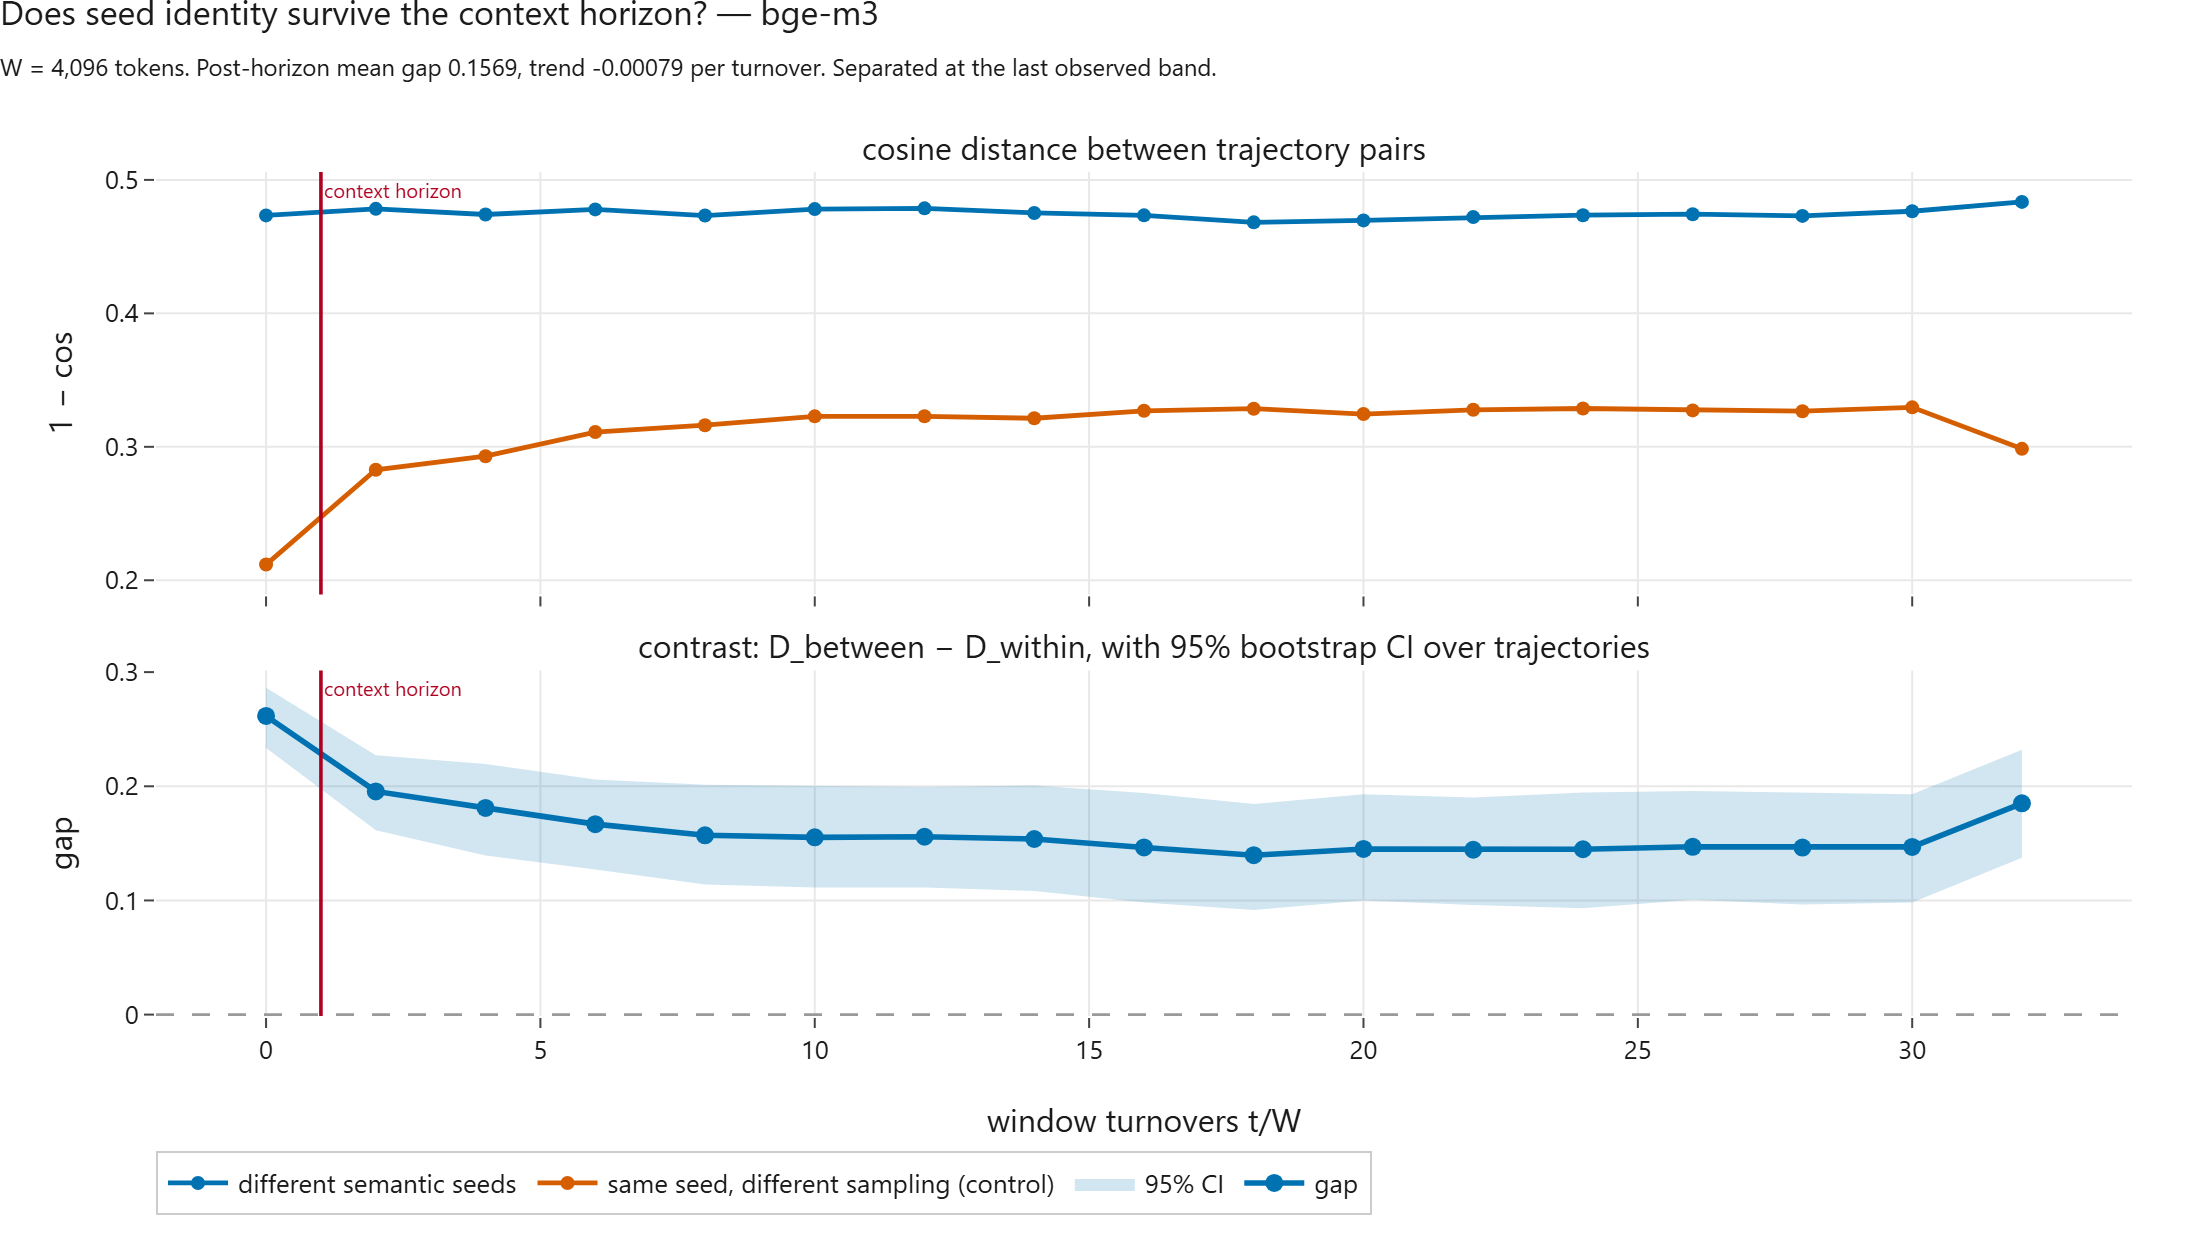
\includegraphics[width=0.92\linewidth]{stage-1/separation-bge-m3/seed_separation.png}
  \caption{Этап~1: domain gap против оборота в \texttt{bge-m3} на пилоте из
    $48$ траекторий \texttt{or-qwen3-8b}. Кривая совместима с тем, что % artifacts/stage-1/separation-bge-m3/seed_separation.png @ s1-separation-bge-m3-20260831T074042Z-9bf54fbf
    идентичность семейства seed переживает горизонт на этой панели с
    большинством вырожденных строк. Это не утверждение, что тот же зазор
    существует в незацикленной подвыборке, на другом генераторе или при
    скользящем KV-кэше.
    Данные: \texttt{artifacts/stage-1/separation-bge-m3/seed\_separation.data.parquet}.
    Generate: \texttt{s1-pilot-core-20260830T134147Z-f1cce9ec}.
    Embed: \texttt{s1-embed-pilot-core-20260831T064430Z-f05e6a68}.
    Separation: \texttt{s1-separation-bge-m3-20260831T074042Z-9bf54fbf}.} % artifacts/stage-1/separation-bge-m3/seed_separation.png @ s1-separation-bge-m3-20260831T074042Z-9bf54fbf
  \label{fig:s1-sep}
\end{figure}

\subsection{Этап 2: lock не универсален среди hosted-генераторов}
\label{sec:s2}

Таблица~\ref{tab:s2-rates} сообщает частоты текстовых неподвижных точек на
четырёхмодельной оси при $T{=}0.3$, $W{=}4096$. % artifacts/stage-2/model-axis/rates/fixed_point_rates.csv @ s2-rates-20260901T125506Z-41d2e88e
\texttt{or-gemma-4-31b} --- $0/8$ (CI $[0,0]$). % artifacts/stage-2/model-axis/rates/fixed_point_rates.csv @ s2-rates-20260901T125506Z-41d2e88e
\texttt{or-gpt-oss-120b} --- $8/8$ (CI $[1,1]$), с оговоркой almost-$T$, % artifacts/stage-2/model-axis/rates/fixed_point_rates.csv @ s2-rates-20260901T125506Z-41d2e88e
задокументированной в отчёте этапа~2. % artifacts/stage-2/model-axis/rates/fixed_point_rates.csv @ s2-rates-20260901T125506Z-41d2e88e
\texttt{or-muse-glimmer-30b} --- $2/8$ (CI $[0, 0.625]$); файл частот % artifacts/stage-2/model-axis/rates/fixed_point_rates.csv @ s2-model-axis-20260901T015457Z-ab59afc8
считает неполные траектории, и только две длинные physics-ячейки достигли
целевого $T$. % artifacts/stage-2/model-axis/rates/fixed_point_rates.csv @ s2-model-axis-20260901T015457Z-ab59afc8
\texttt{or-qwen3-8b} на этой руке --- $7/8$ (CI $[0.625, 1]$). % artifacts/stage-2/model-axis/rates/fixed_point_rates.csv @ s2-rates-20260901T125506Z-41d2e88e
\texttt{or-gpt-oss-20b} дал $0/8$ траекторий, достигших целевого % docs/stages/stage-2/REPORT.md @ s2-model-axis-20260901T015457Z-ab59afc8
$T$ (смерти empty-EOS); $2/7$ из CSV частот не используется. % docs/stages/stage-2/REPORT.md @ s2-model-axis-20260901T015457Z-ab59afc8
По файлу model-axis $11/40$ траекторий достигли целевого $T$. % docs/stages/stage-2/REPORT.md @ s2-model-axis-20260901T015457Z-ab59afc8

Рука механизма prefill-versus-raw на \texttt{or-qwen3-8b} не обнаружила
изменения частоты lock, вызванного prefill: $7/8$ против $8/8$, CI разности % docs/stages/stage-2/REPORT.md @ s2-mechanism-20260901T071519Z-dfbb173a
$[-0.375, 0]$. % docs/stages/stage-2/REPORT.md @ s2-mechanism-20260901T071519Z-dfbb173a
Детерминизм провайдера, измеренный как точное совпадение текста на коротком
зонде, составил
$100\%$ (\texttt{or-muse-glimmer-30b}), $60\%$ (\texttt{or-qwen3-8b}), $20\%$ % docs/stages/stage-2/REPORT.md @ s2-audit-determinism-20260901T015221Z-ab59afc8
(\texttt{or-gemma-4-31b}) и $20\%$ (\texttt{or-gpt-oss-120b}). % docs/stages/stage-2/REPORT.md @ s2-audit-determinism-20260901T015221Z-ab59afc8
Поэтому occupancy-этапы не могут трактовать пары реплик как независимые
выборки детерминированного декодера.

Рисунок частот этапа~2 существует только как SVG
(\texttt{artifacts/stage-2/model-axis/rates/fixed\_point\_rate.svg}). % artifacts/stage-2/model-axis/rates/fixed_point_rate.svg @ s2-rates-20260901T125506Z-41d2e88e
Эта рукопись использует CSV-таблицу, а не растеризованную замену.

\begin{table}[t]
  \centering
  \caption{Частоты текстовых неподвижных точек, ось моделей этапа~2, $T{=}0.3$,
    $W{=}4096$. Источник:
    \texttt{artifacts/stage-2/model-axis/rates/fixed\_point\_rates.csv};
    \texttt{s2-rates-20260901T125506Z-41d2e88e}.
    $0/8$ у Gemma --- доказательство существования того, что freeze этапа~1 % artifacts/stage-2/model-axis/rates/fixed_point_rates.csv @ s2-rates-20260901T125506Z-41d2e88e
    не свойство instruct-моделей как класса.} % artifacts/stage-2/model-axis/rates/fixed_point_rates.csv @ s2-rates-20260901T125506Z-41d2e88e
  \label{tab:s2-rates}
  \begin{tabular}{@{}lccc@{}}
    \toprule
    Генератор & $n$ в файле частот & частота lock & 95\% CI \\
    \midrule
    \texttt{or-qwen3-8b} & $8$ & $7/8$ & $[0.625, 1]$ \\ % artifacts/stage-2/model-axis/rates/fixed_point_rates.csv @ s2-rates-20260901T125506Z-41d2e88e
    \texttt{or-gemma-4-31b} & $8$ & $0/8$ & $[0, 0]$ \\ % artifacts/stage-2/model-axis/rates/fixed_point_rates.csv @ s2-rates-20260901T125506Z-41d2e88e
    \texttt{or-gpt-oss-120b} & $8$ & $8/8$ & $[1, 1]$ \\ % artifacts/stage-2/model-axis/rates/fixed_point_rates.csv @ s2-rates-20260901T125506Z-41d2e88e
    \texttt{or-muse-glimmer-30b} & $8$ & $2/8$ & $[0, 0.625]$ \\ % artifacts/stage-2/model-axis/rates/fixed_point_rates.csv @ s2-rates-20260901T125506Z-41d2e88e
    \texttt{or-gpt-oss-20b} & $0$ достигли $T$ & --- & --- \\ % docs/stages/stage-2/REPORT.md @ s2-model-axis-20260901T015457Z-ab59afc8
    \bottomrule
  \end{tabular}
\end{table}

\subsection{Этап 3: валидированного MSM нет; $n_{\mathrm{macro}}$ --- не параметр порядка}
\label{sec:s3}

Этап~3 применил VAMP/PCCA+ к эмбеддингам панели этапа~1 и local-base зонда.
Таблица валидации равномерно отрицательна:
\texttt{validated=0} в каждой ячейке
\texttt{artifacts/stage-3/dynamics/k\_stability.md}. % artifacts/stage-3/dynamics/k_stability.md @ s3-dynamics-20260901T204521Z-f21d5908
Подразумеваемый $n_{\mathrm{macro}}$ нестабилен по $K$ и по пространствам
эмбеддингов. Chapman--Kolmogorov тесты микросостояний не проходят планку
$0.15$. % artifacts/stage-3/dynamics/k_stability.md @ s3-dynamics-20260901T204549Z-b7c4d0c9
Гипотеза H1 (метастабильные семантические состояния как объект MSM) unsupported. Норма Фробениуса тока вероятности, посчитанного на
\emph{микросостояниях}, не есть свидетельство H4 (необратимые токи между
макросостояниями).

Локальный зонд \texttt{gemma-3-1b-pt} при $W{=}256$ дал $8/8$ вырожденных % docs/stages/stage-3/REPORT.md @ s3-local-base-20260901T184812Z-cc80633b
траекторий и $0/8$ строк в регистре рецензента. % docs/stages/stage-3/REPORT.md @ s3-local-base-20260901T184812Z-cc80633b
Эта ячейка --- другое окно, чем occupancy-панель. Она не заполняет
отсутствующую hosted-base ячейку этапа~0 и не лицензирует утверждение
base-versus-instruct при $W{=}4096$.

\subsection{Этап 4: lock до $T{=}1.5$; H5 отсутствует} % artifacts/stage-4/grid/looping_rate_by_cell.csv @ s4-w4096-new-temps-20260904T103121Z-589c8eb1
\label{sec:s4}

Этап~4 пересёк температуру и окно на \texttt{or-qwen3-8b} с $n{=}4$
траекториями на ячейку. % artifacts/stage-4/grid/looping_rate_by_cell.csv @ s4-w4096-new-temps-20260904T103121Z-589c8eb1
Таблица~\ref{tab:s4-loop} суммирует частоты зацикливания. При $T \le 1.0$ и
$W{=}4096$, и $W{=}8192$ дают $4/4$ looping (CI $[1,1]$). % artifacts/stage-4/grid/looping_rate_by_cell.csv @ s4-w4096-new-temps-20260904T103121Z-589c8eb1
При $T{=}1.5$ $W{=}4096$ даёт $0/4$ looping (CI $[0,0]$); $W{=}8192$ --- $2/4$ (CI $[0,1]$). % artifacts/stage-4/grid/looping_rate_by_cell.csv @ s4-w8192-20260904T120057Z-ce82ce55

Чистый MSD $\alpha$ определён только в незацикленных ячейках.
Определённые ячейки --- $T{=}1.5$: при $W{=}4096$, $\alpha = 0.149$ $[0.140, 0.158]$ в % artifacts/stage-4/grid/clean_alpha_by_cell.csv @ s4-w4096-new-temps-20260904T103121Z-589c8eb1
\texttt{bge-m3} и $\alpha = 0.277$ $[0.241, 0.318]$ в % artifacts/stage-4/grid/clean_alpha_by_cell.csv @ s4-w4096-new-temps-20260904T103121Z-589c8eb1
\texttt{qwen3-embed-8b}; % artifacts/stage-4/grid/clean_alpha_by_cell.csv @ s4-w4096-new-temps-20260904T103121Z-589c8eb1
при $W{=}8192$ ($n_{\mathrm{clean}}{=}2$), $\alpha = 0.146$ $[0.086, 0.207]$ в % artifacts/stage-4/grid/clean_alpha_by_cell.csv @ s4-w8192-20260904T120057Z-ce82ce55
\texttt{bge-m3} и $\alpha = 0.247$ $[0.172, 0.322]$ в % artifacts/stage-4/grid/clean_alpha_by_cell.csv @ s4-w8192-20260904T120057Z-ce82ce55
\texttt{qwen3-embed-8b}. % artifacts/stage-4/grid/clean_alpha_by_cell.csv @ s4-w8192-20260904T120057Z-ce82ce55
Все четыре оценки субдиффузионны. Чистого $\alpha$ при низком $T$ нет, поэтому
H5 (незацикленное confined motion в температурном окне) отсутствует, а не
пограничен. Рисунок~\ref{fig:s4-loop} и рисунок~\ref{fig:s4-alpha} ---
закоммиченные фигуры этапа~4. $n{=}4$ --- вся ячейка, а не large-sample
частота.

\begin{table}[t]
  \centering
  \caption{Частота зацикливания по температуре и окну, этап~4,
    \texttt{or-qwen3-8b}, $n{=}4$ на ячейку. Источник:
    \texttt{artifacts/stage-4/grid/looping\_rate\_by\_cell.csv}.
    Пороги degeneracy остаются Jaccard $0.083$ / late $0.0122$.} % artifacts/stage-1/degeneracy/degeneracy_verdicts.meta.json @ s1-degeneracy-20260831T070038Z-b2f6f0c9
  \label{tab:s4-loop}
  \begin{tabular}{@{}lcccc@{}}
    \toprule
    $T$ & $W{=}4096$ looping & CI & $W{=}8192$ looping & CI \\
    \midrule
    $\le 1.0$ & $4/4$ & $[1,1]$ & $4/4$ & $[1,1]$ \\ % artifacts/stage-4/grid/looping_rate_by_cell.csv @ s4-w4096-new-temps-20260904T103121Z-589c8eb1
    $1.5$ & $0/4$ & $[0,0]$ & $2/4$ & $[0,1]$ \\ % artifacts/stage-4/grid/looping_rate_by_cell.csv @ s4-w8192-20260904T120057Z-ce82ce55
    \bottomrule
  \end{tabular}
\end{table}

\begin{figure}[t]
  \centering
  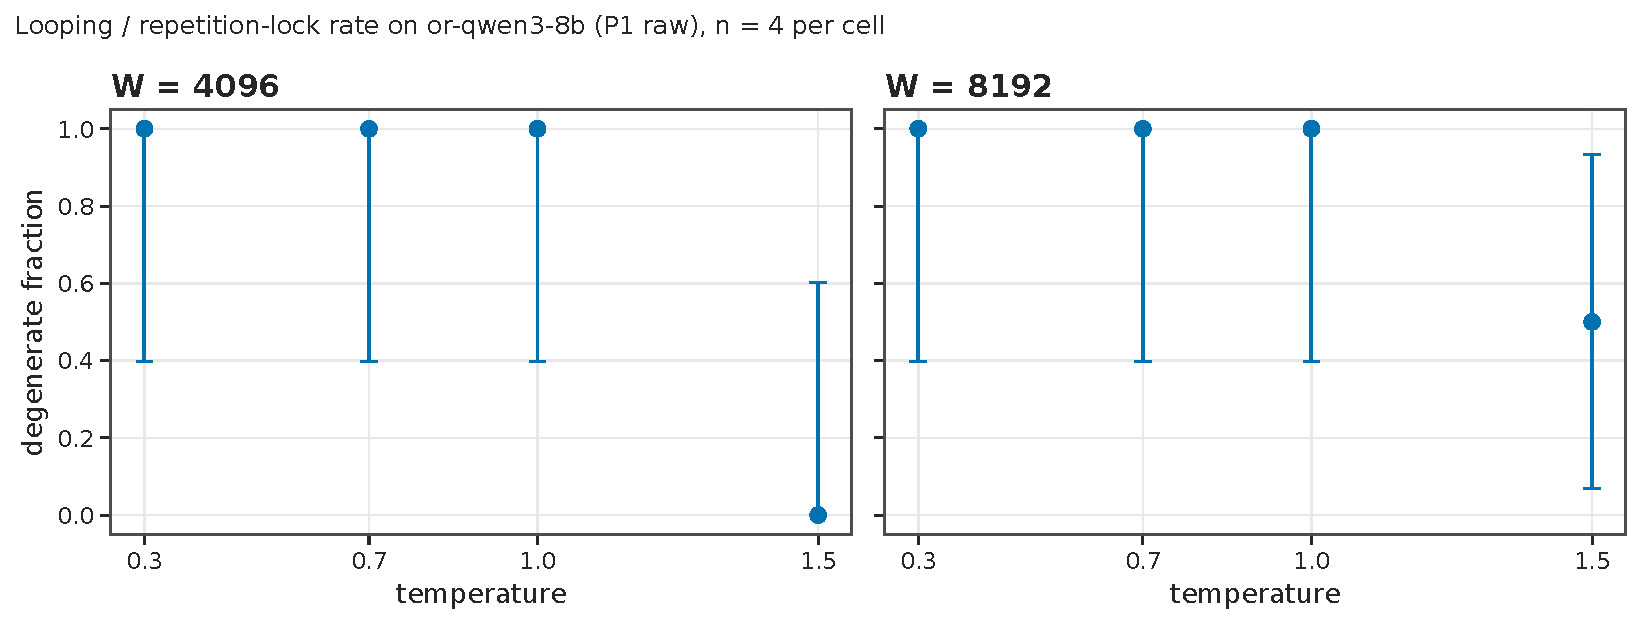
\includegraphics[width=0.85\linewidth]{stage-4/grid/looping_rate_vs_T.pdf}
  \caption{Частота зацикливания против температуры при двух окнах.
    Данные: \texttt{artifacts/stage-4/grid/looping\_rate\_vs\_T.data.parquet}.
    Generate: \texttt{s4-w4096-new-temps-20260904T103121Z-589c8eb1},
    \texttt{s4-w8192-20260904T120057Z-ce82ce55}.
    Ячейка $T{=}1.5$, $W{=}4096$ --- существование незацикленного режима % artifacts/stage-4/grid/looping_rate_vs_T.pdf @ s4-w4096-new-temps-20260904T103121Z-589c8eb1
    на этой модели, а не оценка времени перемешивания.} % artifacts/stage-4/grid/looping_rate_vs_T.pdf @ s4-w4096-new-temps-20260904T103121Z-589c8eb1
  \label{fig:s4-loop}
\end{figure}

\begin{figure}[t]
  \centering
  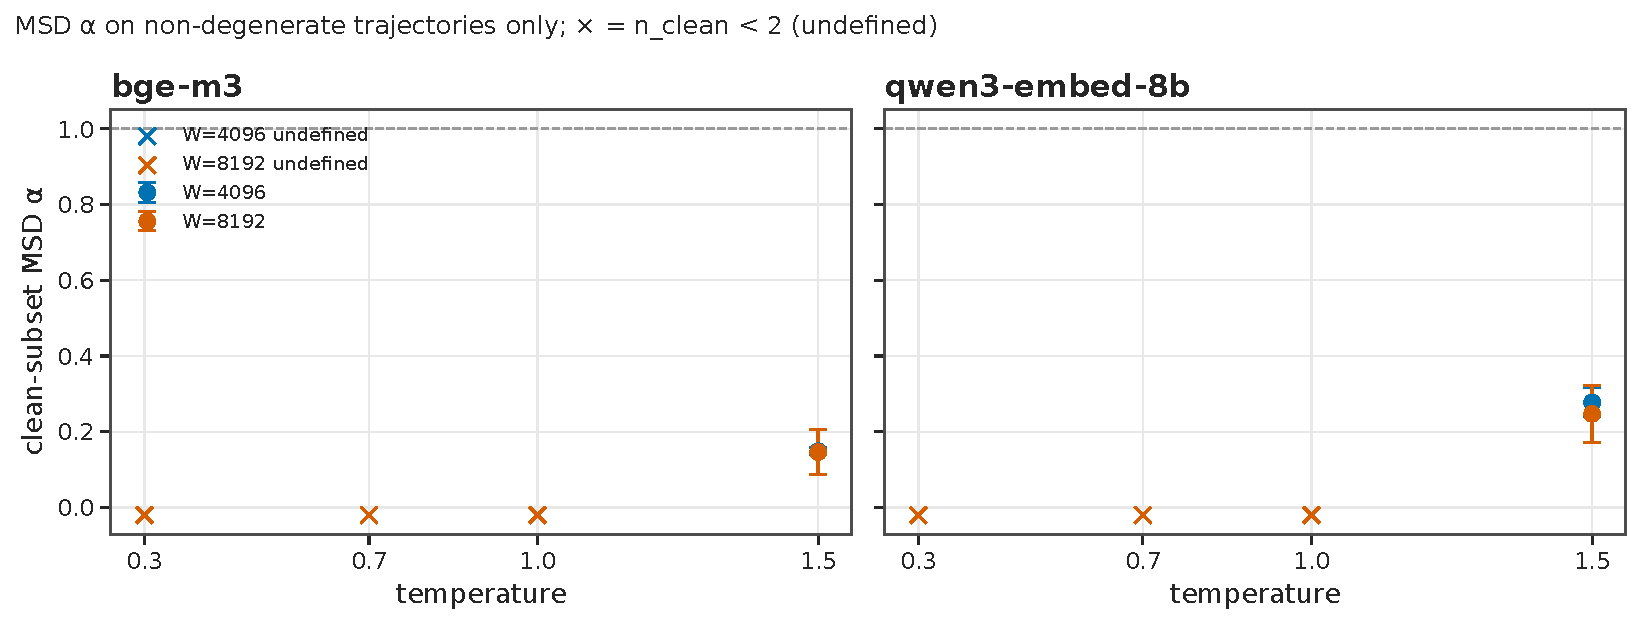
\includegraphics[width=0.85\linewidth]{stage-4/grid/clean_alpha_vs_T.pdf}
  \caption{Чистый MSD $\alpha$ там, где определён (только незацикленные ячейки).
    Данные: \texttt{artifacts/stage-4/grid/clean\_alpha\_vs\_T.data.parquet}.
    Отсутствующие точки при низком $T$ --- отсутствие H5, а не пропуск на графике.} % artifacts/stage-4/grid/clean_alpha_vs_T.pdf @ s4-w4096-new-temps-20260904T103121Z-589c8eb1
  \label{fig:s4-alpha}
\end{figure}

\subsection{Этап 5: last-band occupancy на заблокированной панели}
\label{sec:s5}

Дан lock, этап~5 задаёт два occupancy-вопроса на двадцати восьми
траекториях \texttt{or-qwen3-8b} при $W{=}4096$, $T{=}0.3$, двенадцати оборотах. % docs/stages/stage-5/REPORT.md @ s5-lock-occupancy-20260905T164327Z-6780902f
Generate \texttt{s5-lock-occupancy-20260905T164327Z-6780902f};
embed \texttt{s5-embed-lock-occupancy-20260906T030125Z-eab6e484};
degeneracy \texttt{s5-degeneracy-20260906T030145Z-deb4c3bd}.
Десять доменных seed (включая love) дают по две реплики; четыре twin-seed
дают пары F6.

Occupancy lock: $19/20$ доменных траекторий и $10/10$ доменных seed % artifacts/stage-5/occupancy/lock_rate_by_seed.csv @ s5-degeneracy-20260906T030145Z-deb4c3bd
удовлетворяют правилу текстовой неподвижной точки; love --- $1/2$. % artifacts/stage-5/occupancy/lock_rate_by_seed.csv @ s5-degeneracy-20260906T030145Z-deb4c3bd

F4 в двух пространствах, last band, десять доменных seed, $n{=}20$ траекторий,
$n_{\mathrm{within}}{=}9$ пар после того, как physics seed~1 выпадает из last-band % artifacts/stage-5/occupancy/domain_separation_last_band.csv @ s5-lock-occupancy-20260905T164327Z-6780902f
диагонали:
зазор \texttt{bge-m3} $0.201$, 95\% CI $[0.065, 0.332]$, separated; % artifacts/stage-5/occupancy/domain_separation_last_band.csv @ s5-lock-occupancy-20260905T164327Z-6780902f
зазор \texttt{qwen3-embed-8b} $0.390$, CI $[0.151, 0.593]$, separated. % artifacts/stage-5/occupancy/domain_separation_last_band.csv @ s5-lock-occupancy-20260905T164327Z-6780902f
Этот last-band зазор --- ансамблевая различимость, не recovered prompt
memory (H2).
Рисунок~\ref{fig:s5-dom} показывает зазор против оборота в этих двух пространствах.

F6 (реплика $\Delta$): каждый last-band CI включает $0$ на этой панели. % artifacts/stage-5/occupancy/twin_last_band.csv @ s5-lock-occupancy-20260905T164327Z-6780902f
Operational collapsed --- это утверждение о CI. Это не occupancy одного lock.
Пара Waterloo в \texttt{bge-m3} имеет last-band точечную оценку около
$0.049$, чей CI всё ещё включает $0$. % artifacts/stage-5/occupancy/twin_last_band.csv @ s5-lock-occupancy-20260905T164327Z-6780902f
Фигура twin-$\Delta$ этапа~5 существует только как SVG; трёхпространственная
фигура в разделе~\ref{sec:s6} заменяет её для рукописи.

\begin{figure}[t]
  \centering
  
\includegraphics[width=0.92\linewidth]{stage-5/occupancy/domain_separation_vs_turnover.pdf}
  \caption{Domain gap против оборота в \texttt{bge-m3} и
    \texttt{qwen3-embed-8b} на заблокированной панели этапа~5. Last-band CI
    исключают $0$ сверху в обоих пространствах. Фигура не включает % artifacts/stage-5/occupancy/domain_separation_vs_turnover.pdf @ s5-lock-occupancy-20260905T164327Z-6780902f
    \texttt{gemini-embed-001} (этап~6) и не показывает незацикленную
    подвыборку.
    Данные: \texttt{artifacts/stage-5/occupancy/domain\_separation\_vs\_turnover.data.parquet}.
    Generate: \texttt{s5-lock-occupancy-20260905T164327Z-6780902f}.} % artifacts/stage-5/occupancy/domain_separation_vs_turnover.pdf @ s5-lock-occupancy-20260905T164327Z-6780902f
  \label{fig:s5-dom}
\end{figure}

\subsection{Этап 6: знаки occupancy в третьем пространстве эмбеддингов}
\label{sec:s6}

Этап~6 заново эмбеддировал те же $28$ траекторий в % docs/stages/stage-6/REPORT.md @ s6-embed-third-space-20260906T082301Z-588eff8f
\texttt{gemini-embed-001} и пересобрал F4/F6 в трёх пространствах. Новых
токенов не генерировали. Hosted-траты этапа~6 --- $\$0$. % docs/stages/stage-6/REPORT.md @ s6-embed-third-space-20260906T082301Z-588eff8f
Прогоны эмбеддинга Gemini:
\texttt{s6-embed-third-space-20260906T082301Z-588eff8f},
\texttt{s6-embed-third-space-20260906T082628Z-9077d587}.

Таблица~\ref{tab:s6-f4} сообщает last-band F4. Все три пространства
\texttt{separated} по предрегистрированному правилу CI. Интервал gemini
$[0.029, 0.266]$ исключает $0$ на волоске. % artifacts/stage-6/occupancy/domain_separation_last_band.csv @ s6-embed-third-space-20260906T082301Z-588eff8f
Это проход NHST, не
толстая robustness и не architecture-independence. Три пространства
не согласны по \emph{уровню}: $0.201$ / $0.390$ / $0.150$. % artifacts/stage-6/occupancy/domain_separation_last_band.csv @ s6-embed-third-space-20260906T082301Z-588eff8f
Утверждение --- согласие знака. У physics seed~1 $47$ против $48$ чанков, поэтому % docs/stages/stage-6/REPORT.md @ s6-embed-third-space-20260906T082301Z-588eff8f
его last-band диагональ $D_{\mathrm{within}}$ не определена (NaN) в каждом
пространстве; F4 использует оставшиеся $n_{\mathrm{within}}{=}9$ пар. % docs/stages/stage-6/REPORT.md @ s6-embed-third-space-20260906T082301Z-588eff8f

Таблица~\ref{tab:s6-f6} сообщает last-band F6. Gemini all-pairs $\Delta$ равна
$-0.012$, CI $[-0.286, 0.223]$ (включает $0$). % artifacts/stage-6/occupancy/twin_last_band.csv @ s6-embed-third-space-20260906T082301Z-588eff8f
Пара reactor ни разу не исключила $0$ ни в одном пространстве % artifacts/stage-6/occupancy/twin_last_band.csv @ s6-embed-third-space-20260906T082301Z-588eff8f
($0.008$, CI $[-0.071, 0.087]$ в gemini). % artifacts/stage-6/occupancy/twin_last_band.csv @ s6-embed-third-space-20260906T082301Z-588eff8f
Last-band $\Delta$ Waterloo в gemini равна $-0.031$, CI $[-0.286, 0.223]$; % artifacts/stage-6/occupancy/twin_per_band.csv @ s6-embed-third-space-20260906T082301Z-588eff8f
та же пара в полосе $0$ даёт $0.033$, CI $[0.001, 0.065]$, так что знак % artifacts/stage-6/occupancy/twin_per_band.csv @ s6-embed-third-space-20260906T082301Z-588eff8f
меняется вдоль траектории. % artifacts/stage-6/occupancy/twin_per_band.csv @ s6-embed-third-space-20260906T082301Z-588eff8f
Operational collapsed остаётся «CI включает $0$'', а не «две реплики % artifacts/stage-6/occupancy/twin_per_band.csv @ s6-embed-third-space-20260906T082301Z-588eff8f
occupy one lock».

Рисунок~\ref{fig:s6-f4} и рисунок~\ref{fig:s6-f6} --- трёхпространственные
фигуры этапа~6. Рисунок~\ref{fig:s6-heat} --- last-band матрица косинусных
дистанций в пространстве gemini. Это иллюстрация попарных дистанций, не
число кластеров и не 2-D проекция, использованная как свидетельство.

Протокольная диагностика той же панели, не заголовочный результат: доменные
траектории тратят среднюю долю заполнения $0.853$, 95\% CI $[0.756, 0.936]$, % artifacts/stage-5/occupancy/protocol_by_quarter.csv @ s5-lock-occupancy-20260905T164327Z-6780902f
в последней четверти, при средней доле stop-токенов $0.359$. % artifacts/stage-5/occupancy/protocol_by_quarter.csv @ s5-lock-occupancy-20260905T164327Z-6780902f
P1 fill --- конфаунд, который надо назвать, а не измерение скользящего окна.

\begin{table}[t]
  \centering
  \caption{F4 last-band domain gap, десять доменных seed, $n{=}20$,
    $n_{\mathrm{within}}{=}9$. Источник: % CI excludes $0$ from above.} % artifacts/stage-6/occupancy/domain_separation_last_band.csv @ s6-embed-third-space-20260906T082301Z-588eff8f
    \texttt{artifacts/stage-6/occupancy/domain\_separation\_last\_band.csv}.
    Generate: \texttt{s5-lock-occupancy-20260905T164327Z-6780902f}.
    Gemini embeds: \texttt{s6-embed-third-space-20260906T082301Z-588eff8f},
    \texttt{s6-embed-third-space-20260906T082628Z-9077d587}.
    Separated означает, что 95\% CI исключает $0$ сверху.} % artifacts/stage-6/occupancy/domain_separation_last_band.csv @ s6-embed-third-space-20260906T082301Z-588eff8f
  \label{tab:s6-f4}
  \begin{tabular}{@{}lccc@{}}
    \toprule
    Пространство & gap & 95\% CI & separated \\
    \midrule
    \texttt{bge-m3} & $0.201$ & $[0.065, 0.332]$ & yes \\ % artifacts/stage-6/occupancy/domain_separation_last_band.csv @ s5-lock-occupancy-20260905T164327Z-6780902f
    \texttt{qwen3-embed-8b} & $0.390$ & $[0.151, 0.593]$ & yes \\ % artifacts/stage-6/occupancy/domain_separation_last_band.csv @ s5-lock-occupancy-20260905T164327Z-6780902f
    \texttt{gemini-embed-001} & $0.150$ & $[0.029, 0.266]$ & yes \\ % artifacts/stage-6/occupancy/domain_separation_last_band.csv @ s6-embed-third-space-20260906T082301Z-588eff8f
    \bottomrule
  \end{tabular}
\end{table}

\begin{table}[t]
  \centering
  \caption{F6 last-band реплика $\Delta$, operational collapsed $=$ CI
    включает $0$. Источник: % artifacts/stage-6/occupancy/twin_last_band.csv @ s6-embed-third-space-20260906T082301Z-588eff8f
    \texttt{artifacts/stage-6/occupancy/twin\_last\_band.csv}.
    Эта таблица --- не occupancy одного lock.} % artifacts/stage-6/occupancy/twin_last_band.csv @ s6-embed-third-space-20260906T082301Z-588eff8f
  \label{tab:s6-f6}
  \begin{tabular}{@{}lccc@{}}
    \toprule
    Срез & $\Delta$ & 95\% CI & CI включает $0$ \\
    \midrule
    gemini, все пары & $-0.012$ & $[-0.286, 0.223]$ & yes \\ % artifacts/stage-6/occupancy/twin_last_band.csv @ s6-embed-third-space-20260906T082301Z-588eff8f
    reactor, gemini & $0.008$ & $[-0.071, 0.087]$ & yes \\ % artifacts/stage-6/occupancy/twin_last_band.csv @ s6-embed-third-space-20260906T082301Z-588eff8f
    waterloo, gemini last band & $-0.031$ & $[-0.286, 0.223]$ & yes \\ % artifacts/stage-6/occupancy/twin_last_band.csv @ s6-embed-third-space-20260906T082301Z-588eff8f
    waterloo, gemini полоса $0$ & $0.033$ & $[0.001, 0.065]$ & no \\ % artifacts/stage-6/occupancy/twin_per_band.csv @ s6-embed-third-space-20260906T082301Z-588eff8f
    \bottomrule
  \end{tabular}
\end{table}

\begin{figure}[t]
  \centering
  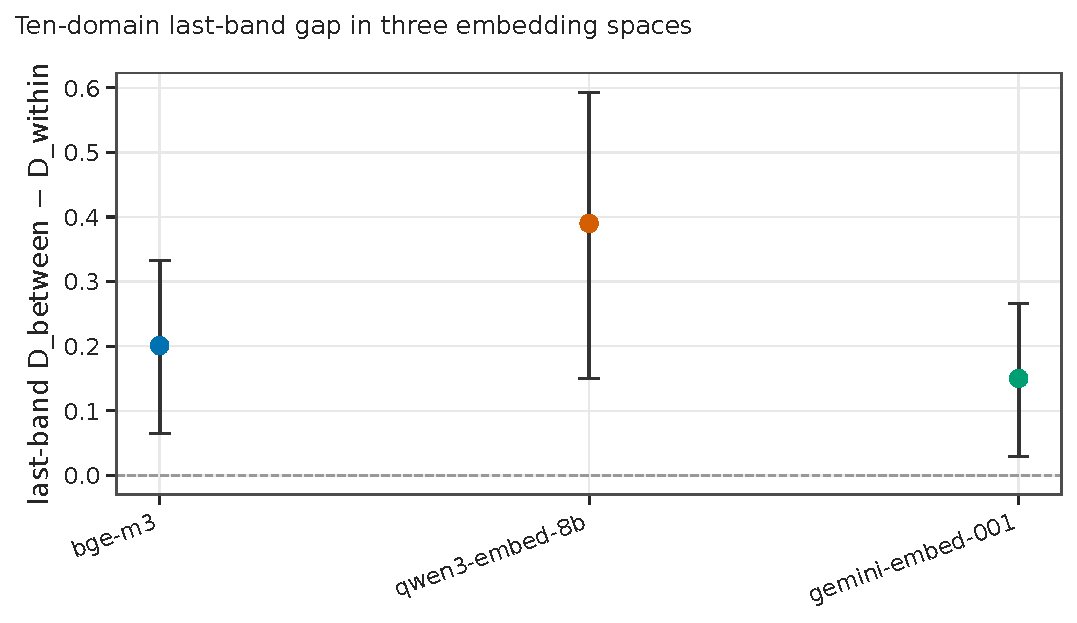
\includegraphics[width=0.92\linewidth]{stage-6/occupancy/domain_gap_three_spaces.pdf}
  \caption{F4 domain gap против оборота в трёх пространствах эмбеддингов на
    тех же $28$ траекториях \texttt{or-qwen3-8b}. Last-band CI исключают $0$ % artifacts/stage-6/occupancy/domain_gap_three_spaces.pdf @ s6-embed-third-space-20260906T082301Z-588eff8f
    во всех трёх пространствах; gemini --- волосок. Уровни $0.201$ / $0.390$ / % artifacts/stage-6/occupancy/domain_gap_three_spaces.pdf @ s6-embed-third-space-20260906T082301Z-588eff8f
    $0.150$ не взаимозаменяемы. % artifacts/stage-6/occupancy/domain_gap_three_spaces.pdf @ s6-embed-third-space-20260906T082301Z-588eff8f
    Данные: \texttt{artifacts/stage-6/occupancy/domain\_gap\_three\_spaces.data.parquet}.} % artifacts/stage-6/occupancy/domain_gap_three_spaces.pdf @ s6-embed-third-space-20260906T082301Z-588eff8f
  \label{fig:s6-f4}
\end{figure}

\begin{figure}[t]
  \centering
  
\includegraphics[width=0.92\linewidth]{stage-6/occupancy/twin_delta_vs_turnover.pdf}
  \caption{F6 реплика $\Delta$ против оборота в трёх пространствах.
    Last-band CI включают $0$. Waterloo в gemini меняет знак от полосы $0$ % artifacts/stage-6/occupancy/twin_delta_vs_turnover.pdf @ s6-embed-third-space-20260906T082301Z-588eff8f
    к последней полосе. Operational collapsed --- это утверждение о CI, а не
    общий lock.
    Данные: \texttt{artifacts/stage-6/occupancy/twin\_delta\_vs\_turnover.data.parquet}.} % artifacts/stage-6/occupancy/twin_delta_vs_turnover.pdf @ s6-embed-third-space-20260906T082301Z-588eff8f
  \label{fig:s6-f6}
\end{figure}

\begin{figure}[t]
  \centering
  
\includegraphics[width=0.72\linewidth]{stage-6/occupancy/last_band_distance_matrix_gemini_embed_001.pdf}
  \caption{Last-band косинусные дистанции в \texttt{gemini-embed-001}
    (иллюстрация попарной матрицы, не число кластеров, не 2-D
    проекция). Physics seed~1 --- неполная last band.
    Данные: \texttt{artifacts/stage-6/occupancy/last\_band\_distance\_matrix\_gemini\_embed\_001.data.parquet}.} % artifacts/stage-6/occupancy/last_band_distance_matrix_gemini_embed_001.pdf @ s6-embed-third-space-20260906T082301Z-588eff8f
  \label{fig:s6-heat}
\end{figure}

\section{Ограничения}
\label{sec:limitations}

\paragraph{P1 против скользящего внимания.}
Каждый afterlife-токен в этой статье получен re-prompt'ом последних $W$
токенов. Нативный скользящий KV-кэш не измерялся. ADR-0017 паркует это
сравнение. Ни одно предложение здесь не есть свидетельство о скользящем
внимании.

\paragraph{Представление.}
Знаки occupancy согласны в \texttt{bge-m3}, \texttt{qwen3-embed-8b} и
\texttt{gemini-embed-001}. Абсолютные зазоры --- нет: $0.201$, $0.390$, $0.150$. % artifacts/stage-6/occupancy/domain_separation_last_band.csv @ s6-embed-third-space-20260906T082301Z-588eff8f
Gemini F4 --- NHST-волосок ($0.029$ на нижней границе CI). % artifacts/stage-6/occupancy/domain_separation_last_band.csv @ s6-embed-third-space-20260906T082301Z-588eff8f
Это не architecture-independence, и этап~6 закрылся на этой формулировке. Мы не
сообщаем ARI/NMI между пространствами; кросс-эмбеддинг проверка --- согласие
знака F4.

\paragraph{Недетерминизм провайдера.}
Частоты точного совпадения на этапе~2 были $100/60/20/20$ процентов на четырёх % docs/stages/stage-2/REPORT.md @ s2-audit-determinism-20260901T015221Z-ab59afc8
hosted-генераторах. % docs/stages/stage-2/REPORT.md @ s2-audit-determinism-20260901T015221Z-ab59afc8
Пары реплик на \texttt{or-qwen3-8b} не гарантированы как независимые
детерминированные выборки.

\paragraph{Конечный горизонт.}
Occupancy использует двенадцать оборотов, а не бесконечный afterlife. % docs/stages/stage-5/REPORT.md @ s5-lock-occupancy-20260905T164327Z-6780902f
Этап~1 достиг
$32$ оборотов на другой панели seed; эта длина не переиспользуется как % docs/stages/stage-1/REPORT.md @ s1-pilot-core-20260830T134147Z-f1cce9ec
время перемешивания occupancy. % docs/stages/stage-1/REPORT.md @ s1-pilot-core-20260830T134147Z-f1cce9ec

\paragraph{Метастабильность против lock.}
Текстовая неподвижная точка --- lock в пространстве токенов. Это не
валидированное макросостояние MSM. Этап~3 нашёл \texttt{validated=0} в каждой
ячейке. % artifacts/stage-3/dynamics/k_stability.md @ s3-dynamics-20260901T204521Z-f21d5908
Эта статья не использует «метастабильные семантические состояния» как
установленную находку.

\paragraph{Один генератор, один протокол, одна температура для occupancy.}
F4 и F6 --- \texttt{or-qwen3-8b}, P1, \texttt{raw\_completion}, served
provider \texttt{Alibaba}, $T{=}0.3$, $W{=}4096$. % docs/stages/stage-5/REPORT.md @ s5-lock-occupancy-20260905T164327Z-6780902f
P1 --- ось re-prompt; \texttt{raw\_completion} --- механизм продолжения.
Они не синонимы. Этап~2 уже измерил prefill versus raw на этом генераторе
($7/8$ против $8/8$, CI разности $[-0.375, 0]$); % docs/stages/stage-2/REPORT.md @ s2-mechanism-20260901T071519Z-dfbb173a
та рука --- не occupancy-протокол. % docs/stages/stage-2/REPORT.md @ s2-mechanism-20260901T071519Z-dfbb173a
Этап~2 уже показывает генератор, у которого частота lock равна $0/8$. % artifacts/stage-2/model-axis/rates/fixed_point_rates.csv @ s2-rates-20260901T125506Z-41d2e88e
Этап~4 уже показывает $T{=}1.5$, $W{=}4096$ с $0/4$ looping. % artifacts/stage-4/grid/looping_rate_by_cell.csv @ s4-w4096-new-temps-20260904T103121Z-589c8eb1
Эти ячейки --- не occupancy-измерения.

\paragraph{Реплики $n{=}2$.}
У каждого доменного seed две траектории. CI F6 широкие. CI, включающий
$0$, может быть underpowered non-detection. % artifacts/stage-6/occupancy/domain_separation_last_band.csv @ s6-embed-third-space-20260906T082301Z-588eff8f

\paragraph{Волосок F4 и physics seed~1.}
Нижняя граница last-band F4 gemini равна $0.029$. % artifacts/stage-6/occupancy/domain_separation_last_band.csv @ s6-embed-third-space-20260906T082301Z-588eff8f
Last-band
$D_{\mathrm{within}}$ physics seed~1 равна NaN из-за несовпадения $47$ против $48$ чанков. % docs/stages/stage-6/REPORT.md @ s6-embed-third-space-20260906T082301Z-588eff8f

\paragraph{F6 --- не один lock.}
Operational collapsed означает, что last-band $\Delta$ CI включает $0$. % artifacts/stage-6/occupancy/twin_per_band.csv @ s6-embed-third-space-20260906T082301Z-588eff8f
Waterloo в gemini меняет знак от полосы $0$ ($0.033$, CI исключает $0$) к % artifacts/stage-6/occupancy/twin_per_band.csv @ s6-embed-third-space-20260906T082301Z-588eff8f
последней полосе ($-0.031$, CI включает $0$). % artifacts/stage-6/occupancy/twin_per_band.csv @ s6-embed-third-space-20260906T082301Z-588eff8f

\paragraph{Degeneracy --- это выборка.}
$19/20$ доменных траекторий --- текстовые неподвижные точки. % artifacts/stage-5/occupancy/lock_rate_by_seed.csv @ s5-degeneracy-20260906T030145Z-deb4c3bd
Occupancy --- факт
о заблокированном тексте, а не о чистой подвыборке, которую отложили.
Пороги $0.083$ / $0.0122$ не двигались; love s1 сохранён. % artifacts/stage-1/degeneracy/degeneracy_verdicts.meta.json @ s1-degeneracy-20260831T070038Z-b2f6f0c9

\paragraph{Нет hosted base-модели.}
Этап~0 не нашёл ни одной. Local-base зонд --- \texttt{gemma-3-1b-pt} при
$W{=}256$, не occupancy-окно. % docs/stages/stage-3/REPORT.md @ s3-local-base-20260901T184812Z-cc80633b

\section{Обсуждение}
\label{sec:discussion}

Что установлено на этом генераторе и протоколе: после того как seed покидает
$W$, типичная траектория при $T{=}0.3$ --- текстовый lock; last-band центроиды
по-прежнему показывают ансамблевый domain gap по десяти доменам seed в трёх
пространствах эмбеддингов (не recovered prompt memory, H2); CI реплики $\Delta$
на last band включают $0$ и не оправдывают заголовок про один lock. % artifacts/stage-6/occupancy/domain_separation_last_band.csv @ s6-embed-third-space-20260906T082301Z-588eff8f

Что не установлено: H1 (валидированные макросостояния MSM); H5 (температурное
окно незацикленного confined motion); мы не можем заявлять architecture-independence
occupancy; результат для языковых моделей как класса; P1 против скользящего
внимания; времена перемешивания; необратимые токи макросостояний.

\citet{zekri2024} остаются правильным нулём единственности. Last-band зазоры
с меткой домена на заблокированной панели совместимы с более чем одной
long-run областью occupancy в пространстве эмбеддингов. Эта совместимость ---
не доказательство, что цепь на уровне токенов имеет несколько стационарных мер.
Это измерение того, где сидят заблокированные траектории после двенадцати
оборотов.

Честное следующее измерение, если оно будет, --- не ещё один эмбеддинг тех же
$28$ строк. Это второй генератор, контраст скользящего кэша или % artifacts/stage-6/occupancy/domain_separation_last_band.csv @ s6-embed-third-space-20260906T082301Z-588eff8f
незацикленная occupancy-панель при $T{=}1.5$. Это припарковано, а не молча % artifacts/stage-6/occupancy/domain_separation_last_band.csv @ s6-embed-third-space-20260906T082301Z-588eff8f
вставлено в эту рукопись.

\section{Воспроизводимость}
\label{sec:repro}

Эксперименты до этапа~6 закрыты на git-коммите \texttt{ad1f244}.
Прогон --- это \texttt{configs/**} плюс этот SHA плюс seed. Сырые траектории
лежат в \texttt{runs/} (gitignored). Публикационные фигуры и tidy-таблицы ---
в \texttt{artifacts/}. Команда
\texttt{afterlife reproduce <run\_id>} --- задуманный путь перевывода
прогона генерации или анализа.

Этап~7 добавляет эту рукопись. Он не добавляет
\texttt{configs/stages/stage7\_*.yaml} и не чеканит фиктивный прогон, чтобы
удовлетворить generate-gate. Hosted-траты этапа~7 равны $\$0$. % docs/stages/stage-7/REPORT.md @ none

Основные \texttt{run\_id}, цитируемые в тексте:

\begin{itemize}
  \item Этап~1 generate: \texttt{s1-pilot-core-20260830T134147Z-f1cce9ec}
  \item Этап~1 degeneracy: \texttt{s1-degeneracy-20260831T070038Z-b2f6f0c9}
  \item Этап~1 embed: \texttt{s1-embed-pilot-core-20260831T064430Z-f05e6a68}
  \item Этап~1 separation: \texttt{s1-separation-bge-m3-20260831T074042Z-9bf54fbf}
  \item Этап~1 geometry: \texttt{s1-geometry-bge-m3-20260831T074420Z-d3c0204a}
  \item Этап~2 model axis: \texttt{s2-model-axis-20260901T015457Z-ab59afc8}
  \item Этап~2 mechanism: \texttt{s2-mechanism-20260901T071519Z-dfbb173a}
  \item Этап~2 determinism: \texttt{s2-audit-determinism-20260901T015221Z-ab59afc8}
  \item Этап~2 rates: \texttt{s2-rates-20260901T125506Z-41d2e88e}
  \item Этап~3 local base: \texttt{s3-local-base-20260901T184812Z-cc80633b}
  \item Этап~3 dynamics: \texttt{s3-dynamics-20260901T204521Z-f21d5908},
        \texttt{s3-dynamics-20260901T204549Z-b7c4d0c9}
  \item Этап~4: \texttt{s4-w4096-new-temps-20260904T103121Z-589c8eb1},
        \texttt{s4-w8192-20260904T120057Z-ce82ce55}
  \item Этап~5 generate: \texttt{s5-lock-occupancy-20260905T164327Z-6780902f}
  \item Этап~5 embed: \texttt{s5-embed-lock-occupancy-20260906T030125Z-eab6e484}
  \item Этап~5 degeneracy: \texttt{s5-degeneracy-20260906T030145Z-deb4c3bd}
  \item Этап~6 gemini: \texttt{s6-embed-third-space-20260906T082301Z-588eff8f},
        \texttt{s6-embed-third-space-20260906T082628Z-9077d587}
\end{itemize}

Канонический английский текст --- \texttt{paper/main.tex}. Этот файл ---
перевод; при расхождении числа и \texttt{run\_id} сверять с английским.

\bibliographystyle{plainnat}
\bibliography{refs}

\end{document}
